\begin{problem}{/images/problems/40_dogs.png}{Dogs Crossing the Bridge}6 dogs weighing 1, 2, 4, 6, 8, and 9 kilograms wish to cross a bridge at night. Also, the capacity of the bridge is 14 kilos and not all of them can cross at the same time. When crossing the bridge, one of them must have a light so that they don't fall off the bridge, but they have only a single light. When several of them pass the bridge together, the duration of the passage is equal to the maximum of their weights. Since not everyone can pass the bridge together, after some  dogs pass the bridge, one of the dogs should bring back the light so that the rest can use it in order to pass the bridge. This process can repeat several times.\\[0.2cm]

What is the fastest way for the dogs to pass the bride?\\[0.2cm]

Link to the problem on Twitter:  \url{https://twitter.com/Riazi_Cafe/status/1705107724927967690}\end{problem}
\begin{solution}
The minimum time  for all dogs to pass the bridge is 24 minutes.\\[0.2cm]

Let us number the dogs by their weight. In the first stage, dogs number 1, 2 and 4 cross the bridge (4 minutes). In the second step, dog 1 will return (1 minute). In the third stage, dogs 6 and 8 cross the bridge (8 minutes).
\begin{center}
	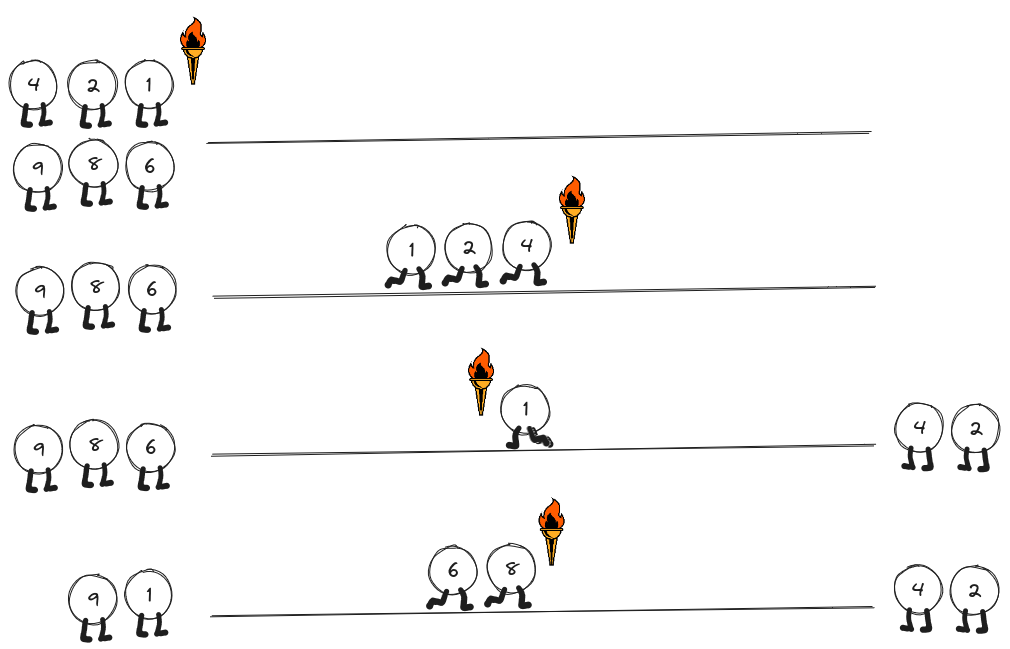
\includegraphics[width=9cm]{/images/problems/40_diagram0.png}
\end{center}

In the fourth stage, dog 2 returns (2 minutes). And finally, in the fifth stage, dogs 1, 2 and 9 will pass the bridge (9 minutes).

\begin{center}
	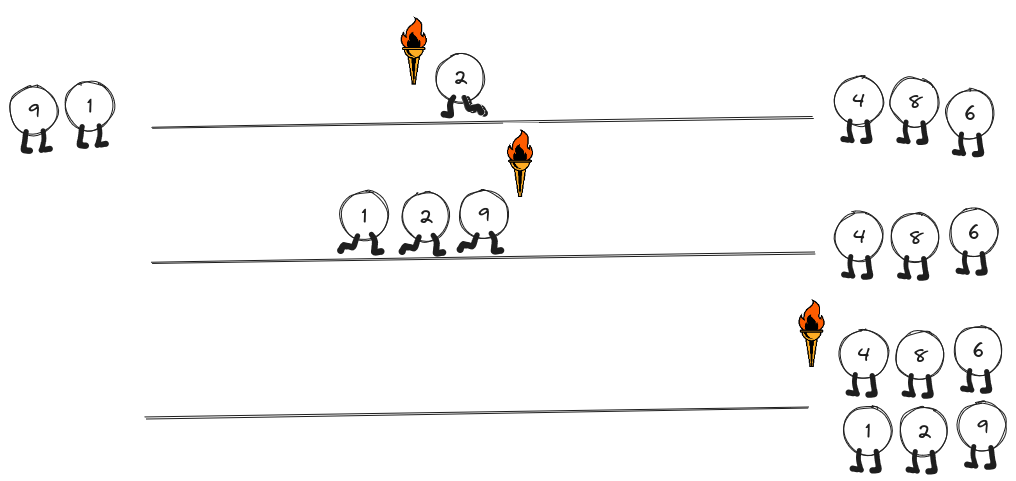
\includegraphics[width=9cm]{/images/problems/40_diagram1.png}
\end{center}

The total amount of time for all dogs to cross the bridge is equal to $4+1+8+2+9 = 24$ minutes.
\end{solution}
